%%% Template originaly created by Karol Kozioł (mail@karol-koziol.net) and modified for ShareLaTeX use

%%%------------------------------------------------------------------------------------------------%%%
%%%------------------------------------%%%     PREAMBLE     %%%------------------------------------%%%
%%%------------------------------------------------------------------------------------------------%%%

\documentclass[twoside=false,a4paper,11pt]{article}

\usepackage[T1]{fontenc}
\usepackage[utf8]{inputenc}
\usepackage{graphicx}
\usepackage{xcolor}

\usepackage{tgtermes}

\usepackage{listings}

\usepackage[
pdftitle={CPSC 471 Final Report},
pdfauthor={Timothy Mealey, University of Calgary},
colorlinks=true,linkcolor=blue,urlcolor=blue,citecolor=blue,bookmarks=true,
bookmarksopenlevel=2]{hyperref}
\usepackage{amsmath,amssymb,amsthm,textcomp}

\usepackage{enumitem}

\usepackage{multicol}
\usepackage{tikz}
\usetikzlibrary{shapes,positioning,calc}
\colorlet{lightgray}{gray!20}

\usepackage{geometry}
\geometry{total={210mm,297mm},
left=25mm,right=25mm,%
bindingoffset=0mm, top=20mm,bottom=20mm}

\linespread{1.3}

\newcommand{\linia}{\rule{\linewidth}{0.5pt}}

% custom theorems if needed
\newtheoremstyle{mytheor}
    {1ex}{1ex}{\normalfont}{0pt}{\scshape}{.}{1ex}
    {{\thmname{#1 }}{\thmnumber{#2}}{\thmnote{ (#3)}}}

\theoremstyle{mytheor}
\newtheorem{defi}{Definition}

% my own titles
\makeatletter
\renewcommand{\maketitle}{
\begin{center}
\vspace{2ex}
{\huge \textsc{\@title}}
\vspace{1ex}
\\
\linia\\
\@author \hfill \@date
\vspace{4ex}
\end{center}
}
\makeatother
%%%

% custom footers and headers
\usepackage{fancyhdr,lastpage}
\pagestyle{fancy}
\lhead{}
\chead{}
\rhead{}
\lfoot{Final Report}
\cfoot{}
\rfoot{Page \thepage\ /\ \pageref*{LastPage}}
\renewcommand{\headrulewidth}{0pt}
\renewcommand{\footrulewidth}{0pt}
%


%%%------------------------------------------------------------------------------------------------%%%
%%%------------------------------------%%%     DOCUMENT     %%%------------------------------------%%%
%%%------------------------------------------------------------------------------------------------%%%

\newcommand{\tuple}[2]{\{ #1 | #2 \}}
\newcommand{\domain}[2]{\{ (#1) | #2 \}}

\newcommand{\quantifier}[2]{(\ensuremath{#1}#2)}
\newcommand{\one}[1]{\quantifier{\exists}{#1}}
\newcommand{\all}[1]{\quantifier{\forall}{#1}}

\begin{document}

\title{CPSC 471 Final Report}
\author{Timothy Mealey, Ben Roberts, Cory Jensen, Scott Saunders}
\date{\today}
\maketitle

\section*{Abstract}

The existing tools for planning semester schedules are decentralized, making them difficult to use together. The goal with this project was to simplify the semester planning process by creating a single tool that encompassed the functionality of the UofC calendar, myUofC course search, degree navigator, and the UofC schedule builder. While we managed to implement most of the desired functionality, we did not implement the degree navigator.

\section*{Introduction}

\subsection*{Problem}

The existing tools for planning semester schedules are decentralized, making them difficult to use together. When building schedules with these tools, it is common to have more than four tabs open in one's internet browser, which is an unnecessarily complicated state for such a simple task. The goal with this project was to simplify the semester planning process by creating a single tool that encompassed the functionality of the UofC calendar, myUofC course search, degree navigator, and the UofC schedule builder.

\subsection*{Implementation}

A course search feature was built which displays course names, descriptions, prerequisites, and whether they are offered in any upcoming or current semesters. It is easily navigable using a searchable sidebar tree organized by faculty, department, and course number - selecting any of which loads that node in the main page. Selecting a node also updates the browser URL to a shareable link, without reloading the page, so that students can easily share their course planning with each other.

Similar to the courses page, the schedule page contains a sidebar tree from which one can choose courses. Differing from the courses page, this sidebar is organized by semester, using a dropdown menu, before dissecting into the different course branches. When one selects a course from the tree, its lectures, tutorials, and labs are added to a sidebar on the right. These sections can then be added to the calendar, located in the centre of the page, from this right side bar. After adding the desired sections to the calendar, the user can save their progress as a schedule.

A login system was started, from which users can be added to the database using an email and password. If a user exists in the database, they can log in using their unique credentials.

\section*{Design}

\subsection*{Users}

``Discuss the different users of your system. Your discussion in this section should be considerably more detailed than what you described for the presentation - this section should describe a complete transaction collection and, consequently, provide a complete picture of the functionality offered by your system.''
%%Put in another file just to handle everything easily.


%\begin{enumerate}

%3 cases: browsing courses (Ie, not necessarily a student), building a schedule, creating an account,

%\item Browsing courses: \\

\subsection*{Browsing Courses}
%
%
%who:   Anyone interested in the courses offered by University of Calgary.
%what:  Course list.
%why:   Has detailed information, provided in a c
  %UofC calendar - no time information.
  %Ours: Has a powerful search, for dept, course number, and course name. %May not be entirely true.
%how:   One visits our page and searches for interesting topics by name, courses in particular, or just simply clicks things.
%
Anyone interested in the courses offered by the University of Calgary, would navigate to our website to evaluate potential classes. They would then search for preferred courses by topic, department, course numbers, or course names. Alternatively one could browse the convenient side-bar for a complete listing. As they select courses, the course info, availability and other information appears in the center of the screen.

\subsection*{Building Schedule}
%\item Building Schedule
%Who:   Anyone interested in attending the University of Calgary.
%what:  Course List and Schedule builder.
%When:  When the data is available!
%why:   Easily build schedules. Easy to enroll via these schedules.
%how:
%
Any Students or Perspective students getting organized for the upcoming semesters, would navigate to our website to construct a class schedule. Powered by the same technology of the dauwtrappen course list, one can find courses and add it to the schedule's selected courses. On this list the user is provided a listing of class times for each section of the class, which they can then select the times they want. If a mistake was made, simply clicking the thing again... Once the user has the schedule to their liking, there are course numbers provided such that the user will be able to use these numbers to enroll directly in those classes via the my.ucalgary.ca Enrollment: add


\subsection*{Login System}
%\item Login System
%Who:   Anyone interested in attending the University of Calgary.
%what:  An account for our system.
%why:   Used to self-organize courses, and curate your own schedules. //Not yet fully implemented.
%how:   Create an account, Verify Account, login!
%

Any new students, prospective students, or returning students, may use the login/account system to curate their own schedules, and checkup on their own interested courses. They would accomplish this by creating an account, (which adds them to the database), and verifying their email. From then on, they are free to login, and see any personalized data sets.
%\end{enumerate}


\subsection*{Entity Relationship Diagram}

\includegraphics[width=\textwidth]{ERDiagram.png}

The red numbers on the diagram mark the changes from the initially presented diagram, and correspond to the list below.

\begin{enumerate}
	\item A prerequisite relation from Course to Course was added.
	\item Removed the ``Course Requirements'' attribute from Degree because it was redundant. It's function is handled by the Requires relation from Degree to Course.
	\item Added the ``Full Name'' attribute to Department because departments have a short code-name as well as a full English name. For example, ``CPSC'' and ``Computer Science.''
	\item A Semester entity type was added, and the Has relation from Semester to Section.
\end{enumerate}

\section*{Implementation}

\subsection*{Relational Schema Diagram}

Below you will find the relational schema diagram, which was created using the algorithm described in class that converts ERDs to RSDs. As you can see, there is a tuple for each entity type and relationship from the ER diagram, with arrows pointing from foreign keys to the primary keys they reference.

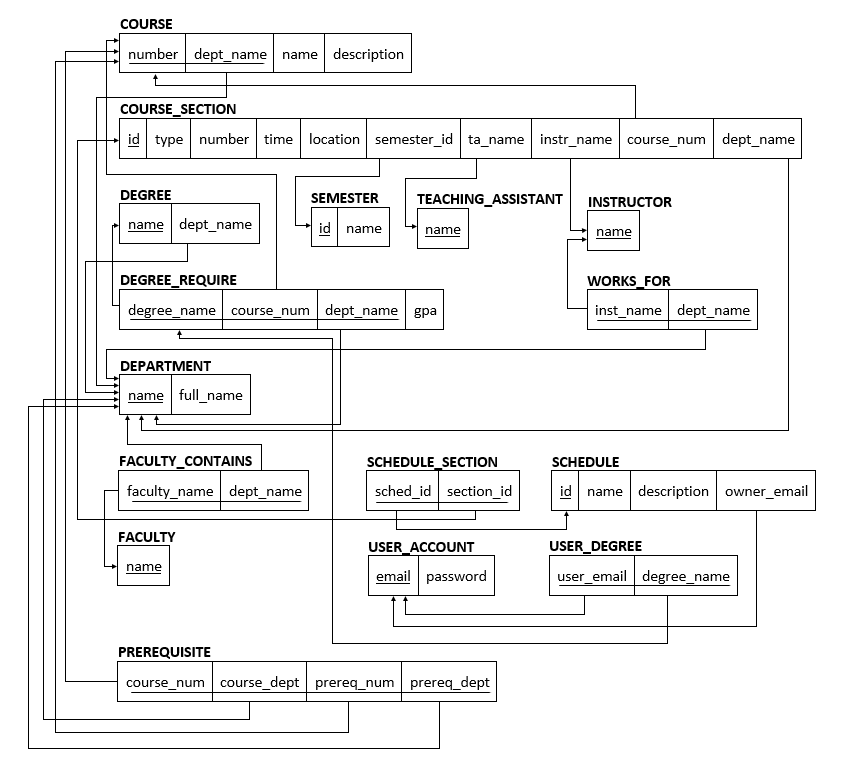
\includegraphics[width=\textwidth]{RelationalSchemaDiagram.png}

During the conversion from the ERD to the RSD, redundancies were found and required information was missing. There were also some interesting constraints put on us by the DBMS that was used. For example, the ``User'' entity was renamed to ``user\_account'' because ``user'' was a reserved keyword.

\subsection*{Database Management System}

``Describe the DBMS you selected for the implementation	of the project, and include the SQL statements for each of the transactions implemented. It is not necessary to discuss these transactions in relational algebra or calculus.''

PostgreSQL is the DBMS used because it is a full-featured SQL implementation with good support and documentation. Here are the SQL queries that were written:

Get a list of all the semesters and the faculties they contain:
\begin{lstlisting}
    SELECT s.*, f.name as fac_name
    FROM
        faculty as f,
        faculty_contains as fc,
        course_section as c,
        semester as s
    WHERE
        c.semester_id=s.id AND
        c.dept_name=fc.dept_name AND
        f.name=fc.faculty_name
    GROUP BY s.id, f.name
\end{lstlisting}

Gets a list of all the semesters:
\begin{lstlisting}
    SELECT s.* FROM semester as s
\end{lstlisting}

Gets a list of all the course sections from a faculty in a semester:
\begin{lstlisting}
    SELECT DISTINCT
        s.*, c.*,
        fc.faculty_name AS fac_name,
        d.full_name AS dept_full_name
    FROM
        course as c,
        faculty_contains as fc,
        course_section as s,
        department as d
    WHERE
        s.semester_id=<SEMESTER_ID> AND
        s.dept_name=fc.dept_name AND
        c.number=s.course_num AND
        c.dept_name=s.dept_name AND
        fc.faculty_name=<FACULTY_NAME> AND
        d.name=s.dept_name
\end{lstlisting}

Gets a list of all the course sections from a faculty:
\begin{lstlisting}
    SELECT DISTINCT
        s.*, c.*,
        fc.faculty_name AS fac_name,
        d.full_name AS dept_full_name
    FROM
        course as c,
        faculty_contains as fc,
        course_section as s,
        department as d
    WHERE
        s.dept_name=fc.dept_name AND
        c.number=s.course_num AND
        c.dept_name=s.dept_name AND
        fc.faculty_name=<FACULTY_NAME> AND
        d.name=s.dept_name
\end{lstlisting}

Checks if a user exists in the database with a given email and password:
\begin{lstlisting}
    SELECT email, password
    FROM user_account
    WHERE email=<EMAIL> AND password=<PASSWORD>
\end{lstlisting}

Checks if a user exists in the database with a given email:
\begin{lstlisting}
    SELECT email
    FROM user_account
    WHERE email=<EMAIL>
\end{lstlisting}

Adds a user account to the database with an email and password:
\begin{lstlisting}
    INSERT INTO user_account
    VALUES (<EMAIL>, <PASSWORD>)
\end{lstlisting}

There are many more INSERT queries in the various scrapers and test-data scripts that populate the database with course information. These have been left out to shorten this document.

\subsection*{User Interface}

``Present a brief description of your interface design, including several screenshots.''

\end{document}
